% =============================================================================
%  마르코프 결정 과정과 최적 정책 — 『밑바닥부터 시작하는 딥러닝 4』 2장 정리
%
%  컴파일:  tectonic -X compile ch02_mdp.tex
%  (XeLaTeX 계열 엔진 + kotex + NanumGothic 필요)
% =============================================================================
\documentclass[11pt,a4paper]{article}

\usepackage{kotex}
\usepackage{amsmath,amssymb}
\usepackage{graphicx}
\usepackage{booktabs}
\usepackage{multirow}
\usepackage{listings}
\usepackage{xcolor}
\usepackage{algorithm}
\usepackage{algpseudocode}
\usepackage[margin=27mm,top=28mm,bottom=28mm]{geometry}
\usepackage[labelsep=period,font=small,labelfont=bf]{caption}
\usepackage{enumitem}
\usepackage[hidelinks]{hyperref}

% ---- 한글 글꼴 -------------------------------------------------------------
\setmainhangulfont{NanumGothic}
\setsanshangulfont{NanumGothic}
\setmonohangulfont[Scale=MatchLowercase]{NanumGothic}

% ---- 한글 캡션 이름 ---------------------------------------------------------
\renewcommand{\figurename}{그림}
\renewcommand{\tablename}{표}
\renewcommand{\refname}{참고문헌}
\renewcommand{\abstractname}{초록}
\renewcommand{\contentsname}{차례}
\floatname{algorithm}{알고리즘}
\renewcommand{\algorithmicrequire}{\textbf{입력:}}
\renewcommand{\algorithmicensure}{\textbf{출력:}}

% ---- 코드 리스팅 -----------------------------------------------------------
\definecolor{codekw}{RGB}{0,86,153}
\definecolor{codecm}{RGB}{112,128,144}
\definecolor{codestr}{RGB}{163,21,21}
\definecolor{codebg}{RGB}{249,249,250}
% 주의: listings는 라틴 문자를 단어 단위로 버퍼링했다가 출력하는데, kotex 환경에서
% 한글이 섞이면 버퍼가 한글 뒤에 flush되어 글자 순서가 뒤바뀐다("q에" -> "에q").
% 그래서 한글 주석은 escapeinside 구간에서 일반 조판 모드로 넘겨 처리한다.
\lstdefinestyle{py}{
  language=Python,
  escapeinside={<@}{@>},
  basicstyle=\ttfamily\small,
  keywordstyle=\color{codekw}\bfseries,
  commentstyle=\color{codecm}\itshape,
  stringstyle=\color{codestr},
  backgroundcolor=\color{codebg},
  frame=single,
  rulecolor=\color{black!25},
  framesep=5pt,
  columns=fullflexible,
  keepspaces=true,
  showstringspaces=false,
  breaklines=true,
  captionpos=b,
  numbers=none,
  aboveskip=1.1em,
  belowskip=0.6em,
}
\lstset{style=py}
\renewcommand{\lstlistingname}{코드}

% ---- 그림 경로 -------------------------------------------------------------
\graphicspath{{../../images/figures/}{../../images/equations/}{../images/}}

% ---- 편의 매크로 -----------------------------------------------------------
\newcommand{\E}{\mathbb{E}}
\newcommand{\Sset}{\mathcal{S}}
\newcommand{\Aset}{\mathcal{A}}
\newcommand{\Lone}{\texttt{L1}}
\newcommand{\Ltwo}{\texttt{L2}}
\newcommand{\bookfig}[1]{\textit{출처: 원서 그림 #1.}}
\newcommand{\cmt}[1]{\textcolor{codecm}{#1}}   % 리스팅 안의 한글 주석

\title{\bfseries 마르코프 결정 과정과 최적 정책\\[2mm]
\large 상태가 개입할 때 무엇이 달라지는가: 할인율의 역할과 전수 탐색의 한계}
\author{sajacaros\\\small \texttt{sajacall82@naver.com}}
\date{2026년 8월 16일}

\begin{document}
\maketitle

\begin{abstract}
\noindent
밴디트 문제에서는 에이전트의 행동이 환경의 상태를 바꾸지 않으므로 ``어떤 행동이 좋은가''만 물으면
되었다. \emph{마르코프 결정 과정}(Markov Decision Process, MDP)은 이 가정을 걷어낸다. 행동이 다음에
마주할 상황을 바꾸는 순간, 눈앞의 보상이 아니라 앞으로 받을 보상의 총합을 기준으로 행동해야 하고,
질문은 ``어떤 상태에서 어떤 행동이 좋은가''로 바뀐다.
본고는 MDP를 상태 집합, 행동 집합, 상태 전이 확률, 보상 함수, 정책의 다섯 요소로 정식화하고,
목표를 수익 $G_t$의 기댓값인 상태 가치 함수 $v_\pi(s)$로 정의한 뒤, 모든 상태에서 동시에 최적인
정책이 존재한다는 MDP의 핵심 성질에 이른다.
원서\cite{dlfs4} 2장은 수식 중심이어서 실행 가능한 코드를 제공하지 않는다. 본고는 2.4절의 두 칸짜리
그리드 월드를 소재로 개념을 코드로 확인할 수 있는 예제 세 편을 구성하고, 여기에 세 가지 정량 분석을
더하였다.
첫째, 할인율 $\gamma$가 수행하는 두 역할을 분리하여 \emph{유효 지평선} $1/(1-\gamma)$와 \emph{절단 오차
상한} $\gamma^N R_{\max}/(1-\gamma)$로 각각 정량화하고, 예제의 지평선 $N=500$이 왜 사실상 무한 걸음과
같은지를 보인다.
둘째, 네 가지 결정적 정책의 상태 가치를 닫힌 형태로 유도하여 수치 결과를 독립적으로 검증하고,
이 환경의 최적 정책이 모든 $\gamma\in[0,1)$에 대해 불변임을 증명한다.
셋째, 그럼에도 $\gamma$가 최적 정책을 바꿀 수 있음을 원서 그림 2-3의 세계에서 보이고, 그 임계값이
정확히 $\gamma=0.4$임을 계산한다. 이는 ``눈앞의 보상만 보면 틀린다''는 2장의 문제의식에 구체적인
숫자를 부여한다.

\vspace{2mm}
\noindent\textbf{주제어:} 강화 학습, 마르코프 결정 과정, 마르코프 성질, 수익, 할인율, 상태 가치 함수,
최적 정책
\end{abstract}

\tableofcontents
\vspace{4mm}

% =============================================================================
\section{서론}
% =============================================================================

\subsection{밴디트 문제에서 MDP로}

앞 장에서 다룬 밴디트 문제\cite{ch01}는 강화 학습의 가장 단순한 형태였다. 어느 슬롯머신을 당기든
다음에 마주하는 상황은 늘 같았기 때문에, 사실상 상태가 존재하지 않았고 에이전트는 ``어떤 행동이
좋은가''만 물으면 되었다. 행동 가치 $q(A)=\E[R\mid A]$ 하나만 잘 추정하면 문제가 풀렸다.

\emph{마르코프 결정 과정}(Markov Decision Process, 이하 MDP)은 이 가정을 걷어낸다. 에이전트가 행동하면
환경의 상태가 바뀌고, 바뀐 상태에서 다시 행동해야 한다. 그림~\ref{fig:grid-intro}의 그리드 월드가
그 최소 예다. 칸이 다섯 개인 1차원 세계에서 에이전트는 한 걸음에 한 칸씩 좌우로 움직이며, 왼쪽 끝의
사과는 $+1$, 오른쪽 끝의 폭탄은 $-2$의 보상을 준다.

\begin{figure}[htbp]
\centering
\includegraphics[width=0.62\linewidth]{{fig 2-1}.png}
\caption{MDP 문제의 예: 그리드 월드. 에이전트가 어디로 움직이느냐에 따라 다음에 놓이는 칸이 달라진다.
\bookfig{2-1}}
\label{fig:grid-intro}
\end{figure}

이 그림만 보면 답은 명백하다. 왼쪽으로 두 칸 가서 사과를 먹으면 된다. 그러나 칸의 배치를 조금 바꾸면
사정이 달라진다. 그림~\ref{fig:grid-alt}에서는 폭탄 너머에 사과 여섯 개$(+6)$가 놓여 있다. 폭탄을
밟는 손해를 감수하고 지나가면 $-2+6=+4$를 얻으므로, 왼쪽 사과 $+1$보다 이득일 수 있다.

\begin{figure}[htbp]
\centering
\includegraphics[width=0.62\linewidth]{{fig 2-3}.png}
\caption{또 다른 세계. 폭탄$(-2)$ 너머에 더 큰 보상$(+6)$이 있다. 눈앞의 보상만 비교하면 최적 행동을
놓친다. \bookfig{2-3}}
\label{fig:grid-alt}
\end{figure}

두 그림의 대비가 이 장 전체의 문제의식이다. 상태가 개입하는 순간, \emph{지금 받을 보상}이 아니라
\emph{앞으로 받을 보상의 총합}을 기준으로 행동해야 한다. ``이득일 수 있다''고 조건부로 쓴 것도
그래서다. $+6$이 두 걸음 뒤에 온다면 그것을 얼마나 가치 있게 볼 것인가에 따라 답이 달라지는데,
그 판단을 맡는 것이 3절에서 도입할 할인율 $\gamma$다. 본고는 \S\ref{sec:gamma-flip}에서 이 세계의
임계값이 정확히 $\gamma=0.4$임을 계산하여, 그림~\ref{fig:grid-alt}이 정성적으로 말하는 바에 숫자를
붙인다.

\subsection{본고의 구성과 기여}

2절에서 MDP를 다섯 요소로 정식화하고 마르코프 성질을 정리한다. 3절에서 목표를 수익과 상태 가치
함수로 정의하고 최적 정책의 존재를 논한다. 4절은 두 칸짜리 그리드 월드에 이를 적용한 실험이며,
5절에서 할인율이 최적 정책을 바꾸는 경우를 다룬다.

원서 2장은 수식 중심이어서 실행 가능한 코드를 제공하지 않는다. 본고가 추가한 것은 다음 세 가지다.

\begin{enumerate}[leftmargin=*,itemsep=2pt]
  \item \textbf{할인율의 두 역할 분리}(\S\ref{sec:gamma}). $\gamma$는 ``얼마나 멀리 보는가''와
        ``수익이 수렴하는가''라는 서로 다른 두 일을 동시에 한다. 전자를 유효 지평선 $1/(1-\gamma)$로,
        후자를 절단 오차 상한 $\gamma^N R_{\max}/(1-\gamma)$로 각각 정량화하고, 예제가 쓰는
        $N=500$이 왜 사실상 무한 걸음과 같은지를 수치로 확인한다.
  \item \textbf{닫힌 형태 해에 의한 검증}(\S\ref{sec:closed-form}). 네 가지 결정적 정책의 상태 가치를
        등비급수로 직접 풀어, 수치 계산 결과를 독립적으로 검증한다. 나아가 이 환경의 최적 정책이
        모든 $\gamma\in[0,1)$에 대해 불변임을 보인다.
  \item \textbf{$\gamma$가 최적 정책을 바꾸는 임계값}(\S\ref{sec:gamma-flip}). 위 결과는 두 칸 세계의
        특수성이다. 원서 그림 2-3의 세계에서는 $\gamma=0.4$를 경계로 최적 행동이 뒤집힘을 보여,
        $\gamma$가 단순한 수렴 장치가 아니라 문제의 답을 결정하는 요소임을 밝힌다.
\end{enumerate}

% =============================================================================
\section{문제 설정: MDP의 다섯 요소}
% =============================================================================

\subsection{에이전트와 환경의 상호작용}

MDP에서 에이전트와 환경은 시간 단계마다 다음을 주고받는다.

\begin{figure}[htbp]
\centering
\includegraphics[width=0.52\linewidth]{{fig 2-4}.png}
\caption{MDP의 사이클. 밴디트와 달리 환경에서 나오는 화살표가 \emph{둘}이다. 보상 $R_t$와 함께 다음
상태 $S_{t+1}$이 돌아온다. \bookfig{2-4}}
\label{fig:mdp-cycle}
\end{figure}

한 시간 단계 $t$의 흐름은 다음과 같다. 에이전트는 상태 $S_t$를 보고 행동 $A_t$를 고른다. 환경은
보상 $R_t$를 주고 상태를 $S_{t+1}$로 바꾼다. 시간을 하나 진행시켜 이를 반복한다. 이하에서 대문자는
확률 변수($S_t$, $A_t$, $R_t$)를, 소문자는 구체적인 값($s$, $a$, $r$)을 가리킨다.

MDP를 완전히 정의하려면 표~\ref{tab:mdp-elements}의 다섯 가지가 필요하다. 앞의 넷이 환경에 속하고,
마지막 하나만이 에이전트의 것이다. 강화 학습이 바꿀 수 있는 것은 오직 정책뿐이라는 사실이 여기서
분명해진다.

\begin{table}[htbp]
\centering
\caption{MDP를 정의하는 다섯 요소}
\label{tab:mdp-elements}
\small
\begin{tabular}{@{}lll@{}}
\toprule
기호 & 이름 & 누구의 것인가 \\
\midrule
$\Sset$          & 상태의 집합       & 환경 \\
$\Aset$          & 행동의 집합       & 환경 \\
$p(s'\mid s,a)$  & 상태 전이 확률    & 환경 \\
$r(s,a,s')$      & 보상 함수         & 환경 \\
$\pi(a\mid s)$   & 정책              & \textbf{에이전트} \\
\bottomrule
\end{tabular}
\end{table}

여기에 수익을 계산할 때 쓰는 할인율 $\gamma$가 더해진다. $\gamma$는 환경의 성질이라기보다 ``무엇을
목표로 삼을 것인가''를 정하는 설계자의 선택에 가깝다는 점에서 나머지와 성격이 다르며, 이 구분은
\S\ref{sec:gamma-flip}에서 다시 문제가 된다.

\subsection{상태 전이와 마르코프 성질}

같은 상태에서 같은 행동을 해도 결과가 하나로 정해지지 않을 수 있다.

\begin{figure}[htbp]
\centering
\includegraphics[width=0.86\linewidth]{{fig 2-5}.png}
\caption{결정적 전이(왼쪽)와 확률적 전이(오른쪽). 오른쪽에서는 \texttt{Left}를 골라도 $0.1$의 확률로
오른쪽으로 밀린다. \bookfig{2-5}}
\label{fig:transition}
\end{figure}

결정적 전이는 함수 하나로 충분하다: $s'=f(s,a)$. 확률적 전이는 \emph{상태 전이 확률}
$p(s'\mid s,a)$로 표현한다. 그림~\ref{fig:transition-prob}이 그 예로, $\texttt{L3}$에서 \texttt{Left}를
골랐을 때 $\texttt{L2}$로 갈 확률이 $0.9$, 제자리에 머물 확률이 $0.1$이다. 한 행의 합이 $1$이 되는
것은 이것이 확률분포이기 때문이다.

\begin{figure}[htbp]
\centering
\includegraphics[width=0.86\linewidth]{{fig 2-6}.png}
\caption{상태 전이 확률의 예. 각 $(s,a)$마다 다음 상태에 대한 확률분포가 하나씩 정의된다.
\bookfig{2-6}}
\label{fig:transition-prob}
\end{figure}

여기서 결정적으로 중요한 것은 $p(s'\mid s,a)$의 조건부에 $S_{t-1}$이나 $A_{t-3}$ 같은 과거가 등장하지
않는다는 사실이다. 다음 상태가 \emph{직전의 상태와 행동만으로} 정해지는 이 성질을
\emph{마르코프 성질}(Markov property)이라 하고, 형식적으로는 다음과 같이 쓴다.
\begin{equation}
  P\bigl(S_{t+1}=s' \mid S_t, A_t, S_{t-1}, A_{t-1}, \dots, S_0, A_0\bigr)
  = P\bigl(S_{t+1}=s' \mid S_t, A_t\bigr).
  \label{eq:markov}
\end{equation}

이런 가정을 두는 이유는 실용적이다. 과거 전체를 조건에 넣으면 조건의 가짓수가 시간에 따라 무한히
늘어나 다룰 수 없게 된다. 식~\eqref{eq:markov}은 그 대신 ``필요한 정보는 모두 현재 상태에 담아
둔다''고 약속한다. 예컨대 속도가 결과에 영향을 준다면 위치만이 아니라 $(\text{위치},\text{속도})$를
하나의 상태로 정의하면 된다. 즉 마르코프 성질은 세계에 대한 강한 주장이라기보다 \emph{상태를 어떻게
설계할 것인가}에 대한 요구 사항이며, 이 요구를 만족하도록 세운 문제가 곧 \emph{마르코프} 결정
과정이다.

\subsection{보상 함수}

\emph{보상 함수} $r(s,a,s')$는 상태 $s$에서 행동 $a$를 취해 $s'$에 도착했을 때 받는 보상이다.

\begin{figure}[htbp]
\centering
\includegraphics[width=0.78\linewidth]{{fig 2-7}.png}
\caption{보상 함수의 예. 인수가 셋이라는 점에 유의한다. 어디서 출발했는지, 무엇을 했는지, 어디에
도착했는지를 모두 본다. \bookfig{2-7}}
\label{fig:reward}
\end{figure}

본고는 원서를 따라 보상이 결정적이라고 가정한다. 즉 세 값 $(s,a,s')$이 정해지면 보상이 하나로
정해진다. 보상 자체가 확률적인 경우에도 기댓값 $\E[R_t\mid s,a,s']$로 두면 이후의 논의가 그대로
성립하므로 일반성을 크게 잃지 않는다.

강조할 점은 보상이 \emph{환경이 정하는 값}이라는 사실이다. 에이전트는 보상을 고를 수 없고 받을 뿐이다.
그림~\ref{fig:grid-intro}과 그림~\ref{fig:grid-alt}에서 보았듯, 보상을 어디에 얼마로 배치하느냐가 곧
문제의 정답을 바꾼다. 강화 학습에서 보상 설계가 문제 정의 그 자체인 이유다.

\subsection{정책}

\emph{정책}(policy)은 에이전트가 상태를 보고 행동을 정하는 방식이다.

\begin{figure}[htbp]
\centering
\includegraphics[width=0.86\linewidth]{{fig 2-8}.png}
\caption{결정적 정책(왼쪽)과 확률적 정책(오른쪽). 오른쪽 괄호 안 숫자의 합은 $1$이다.
\bookfig{2-8}}
\label{fig:policy}
\end{figure}

결정적 정책은 함수 $\mu:\Sset\to\Aset$로 $a=\mu(s)$와 같이 쓰고, 확률적 정책은 조건부 분포
$\pi(a\mid s)$로 쓴다. 결정적 정책은 한 행동의 확률이 $1$인 확률적 정책의 특수한 경우이므로, 이하에서는
$\pi(a\mid s)$로 통일한다.

정책이 \emph{현재 상태만} 보고 행동을 정해도 충분한 근거가 바로 마르코프 성질이다. 환경이 현재 상태와
행동만으로 다음을 정하는 이상, 에이전트가 과거를 기억해서 얻을 이득이 없다. 정리하면 MDP의 한 시간
단계는 다음과 같이 진행된다.
\begin{align}
  \text{에이전트:}\quad & A_t \sim \pi(a\mid S_t), \label{eq:agent-step}\\
  \text{환경:}\quad     & S_{t+1} \sim p(s'\mid S_t, A_t), \qquad R_t = r(S_t, A_t, S_{t+1}).
  \label{eq:env-step}
\end{align}

% =============================================================================
\section{목표: 수익과 상태 가치 함수}
% =============================================================================

\subsection{일회성 과제와 지속적 과제}

MDP는 끝이 있는 문제와 없는 문제로 나뉜다. \emph{일회성 과제}(episodic task)는 종료 상태에 도달하면
한 판이 끝나고 처음부터 다시 시작하는 문제로, 한 판을 \emph{에피소드}(episode)라 부른다. 바둑이나 미로
탈출이 여기에 속한다.

\begin{figure}[htbp]
\centering
\includegraphics[width=0.72\linewidth]{{fig 2-9}.png}
\caption{끝이 있는 문제. \texttt{Goal}에 도달하면 에피소드가 끝나고 처음부터 다시 시작한다.
\bookfig{2-9}}
\label{fig:episodic}
\end{figure}

\emph{지속적 과제}(continuing task)는 종료 상태 없이 계속되는 문제다. 재고 관리가 그 예이며, 4절에서
다룰 두 칸짜리 그리드 월드도 여기에 속한다. 이 구분이 중요한 이유는 단순하다. 끝이 없으면 보상을
그냥 더할 수 없다. 총합이 무한대로 발산해 두 정책의 우열을 비교할 수 없게 된다.

\subsection{수익과 할인율}
\label{sec:gamma}

\emph{수익}(return) $G_t$는 시각 $t$ 이후로 받는 보상을 할인해서 모두 더한 값이다.
\begin{equation}
  G_t = R_t + \gamma R_{t+1} + \gamma^2 R_{t+2} + \cdots
      = \sum_{k=0}^{\infty} \gamma^k R_{t+k},
  \qquad 0 \le \gamma \le 1.
  \label{eq:return}
\end{equation}
$\gamma$를 \emph{할인율}(discount rate)이라 한다. 할인율을 두는 이유는 셋이다. 첫째, $\gamma<1$이면
식~\eqref{eq:return}이 등비급수로 억눌려 지속적 과제에서도 유한한 값으로 수렴한다. 둘째, 100걸음 뒤의
사과보다 지금의 사과가 낫다는 상식을 반영한다. 셋째, 먼 미래일수록 예측이 어긋날 가능성이 크다는
불확실성을 반영한다.

식~\eqref{eq:return}에서 즉시 얻어지는 것이 다음 재귀 관계다.
\begin{equation}
  G_t = R_t + \gamma\, G_{t+1}.
  \label{eq:return-recursive}
\end{equation}
식~\eqref{eq:return-recursive}은 본고에서 계산의 도구로만 쓰이지만, 다음 장에서 벨만 방정식이
세워지는 바로 그 자리다. 코드에서는 보상 열을 뒤에서부터 접어 올리는 한 줄로 나타난다.

\begin{lstlisting}[caption={수익의 계산 (\texttt{s01\_mdp.py})},label={lst:return}]
def calc_return(rewards, gamma):
    <@\cmt{"""보상 나열로부터 수익 G를 계산 (뒤에서부터 거꾸로 접어 올린다)"""}@>
    G = 0.0
    for reward in reversed(rewards):
        G = reward + gamma * G  <@\cmt{\# $G_t = R_t + \gamma G_{t+1}$}@>
    return G
\end{lstlisting}

\subsubsection*{[보충] 할인율의 두 역할}

$\gamma$는 서로 다른 두 가지 일을 동시에 한다. 이 둘을 분리해 보면 $\gamma$를 어떻게 고를지가
분명해진다.

\paragraph{역할 1: 유효 지평선.}
$k$걸음 뒤의 보상에는 가중치 $\gamma^k$가 붙는다. 가중치의 총합
\begin{equation}
  \sum_{k=0}^{\infty}\gamma^k = \frac{1}{1-\gamma}
  \label{eq:effective-horizon}
\end{equation}
을 \emph{유효 지평선}(effective horizon)이라 부른다. 에이전트가 사실상 몇 걸음 앞까지 내다보는지를
나타내는 척도다. 표~\ref{tab:horizon}에 몇 가지 값을 정리하였다. $\gamma=0.9$는 대략 10걸음,
$\gamma=0.99$는 100걸음 앞을 보는 에이전트를 뜻한다.

\begin{table}[htbp]
\centering
\caption{할인율에 따른 유효 지평선. 마지막 열은 가중치 $\gamma^k$가 $0.01$ 아래로 떨어지는 걸음 수
$k=\ln(0.01)/\ln\gamma$이다.}
\label{tab:horizon}
\small
\begin{tabular}{@{}lcc@{}}
\toprule
$\gamma$ & 유효 지평선 $1/(1-\gamma)$ & $\gamma^k<0.01$이 되는 $k$ \\
\midrule
$0.0$  & $1.00$   & $0.0$   \\
$0.3$  & $1.43$   & $3.8$   \\
$0.5$  & $2.00$   & $6.6$   \\
$0.7$  & $3.33$   & $12.9$  \\
$0.9$  & $10.00$  & $43.7$  \\
$0.99$ & $100.00$ & $458.2$ \\
\bottomrule
\end{tabular}
\end{table}

\paragraph{역할 2: 절단 오차의 통제.}
무한급수인 식~\eqref{eq:return}을 컴퓨터로 계산하려면 어딘가에서 잘라야 한다. $N$걸음까지만 더한
근사를 $G^{(N)}$이라 하면, 보상의 크기가 $|R|\le R_{\max}$로 유계일 때 절단 오차는 다음으로 억눌린다.
\begin{equation}
  \bigl|G - G^{(N)}\bigr|
  = \Bigl|\sum_{k=N}^{\infty}\gamma^k R_{t+k}\Bigr|
  \;\le\; R_{\max}\sum_{k=N}^{\infty}\gamma^k
  \;=\; \frac{R_{\max}\,\gamma^{N}}{1-\gamma}.
  \label{eq:truncation}
\end{equation}
4절의 예제는 $\gamma=0.9$, $R_{\max}=1$, $N=500$을 쓰므로 오차 상한이
$0.9^{500}/0.1 \approx 1.3\times10^{-22}$이다. 배정밀도 부동소수점의 분해능보다 훨씬 작으므로
$N=500$은 사실상 무한 걸음과 같다. 표~\ref{tab:truncation}이 이를 실측과 함께 보여준다.

\begin{table}[htbp]
\centering
\caption{$\gamma=0.9$에서 절단 걸음 수 $N$에 따른 수익의 근사와 오차. 참값은
$1/(1-\gamma^2)=5.2631578947\ldots$이며, 실측 오차가 모든 행에서 식~\eqref{eq:truncation}의 상한
아래에 있다.}
\label{tab:truncation}
\small
\begin{tabular}{@{}rlll@{}}
\toprule
$N$ & $G^{(N)}$ & 실측 오차 & 상한 $\gamma^N/(1-\gamma)$ \\
\midrule
$1$   & $1.0000000000$ & $4.26\times10^{0}$   & $9.00\times10^{0}$   \\
$2$   & $1.0000000000$ & $4.26\times10^{0}$   & $8.10\times10^{0}$   \\
$5$   & $2.4661000000$ & $2.80\times10^{0}$   & $5.90\times10^{0}$   \\
$10$  & $3.4280082100$ & $1.84\times10^{0}$   & $3.49\times10^{0}$   \\
$50$  & $5.2360327621$ & $2.71\times10^{-2}$  & $5.15\times10^{-2}$  \\
$100$ & $5.2630180979$ & $1.40\times10^{-4}$  & $2.66\times10^{-4}$  \\
$500$ & $5.2631578947$ & $2.67\times10^{-15}$ & $1.32\times10^{-22}$ \\
\bottomrule
\end{tabular}
\end{table}

마지막 행은 따로 읽어야 한다. $N=500$에서 실측 오차 $2.67\times10^{-15}$가 상한
$1.32\times10^{-22}$보다 크지만 이는 식~\eqref{eq:truncation}의 반례가 아니다. 이 지점에서 절단 오차는
이미 배정밀도의 기계 엡실론($\approx 2.2\times10^{-16}$) 아래로 내려갔고, 남은 것은 500번의 덧셈에서
누적된 반올림 오차다. 즉 $N\gtrsim 350$부터는 절단이 아니라 부동소수점 정밀도가 오차를 지배한다.

\paragraph{두 역할의 긴장.}
두 역할은 서로 반대 방향으로 작용한다. 먼 미래를 보려면 $\gamma$를 키워야 하지만, $\gamma$를 키우면
같은 정확도를 얻는 데 필요한 걸음 수가 늘어난다. 식~\eqref{eq:truncation}에서 오차를 $\epsilon$ 아래로
낮추는 데 필요한 걸음 수는
\begin{equation}
  N \;\ge\; \frac{\ln\bigl(\epsilon(1-\gamma)/R_{\max}\bigr)}{\ln\gamma}
\end{equation}
이며, $\gamma\to1$에서 발산한다. 그림~\ref{fig:discount} 오른쪽에서 $\gamma=0.99$의 곡선만이 200걸음
후에도 여전히 상승하고 있는 것이 그 시각적 표현이다.

\begin{figure}[htbp]
\centering
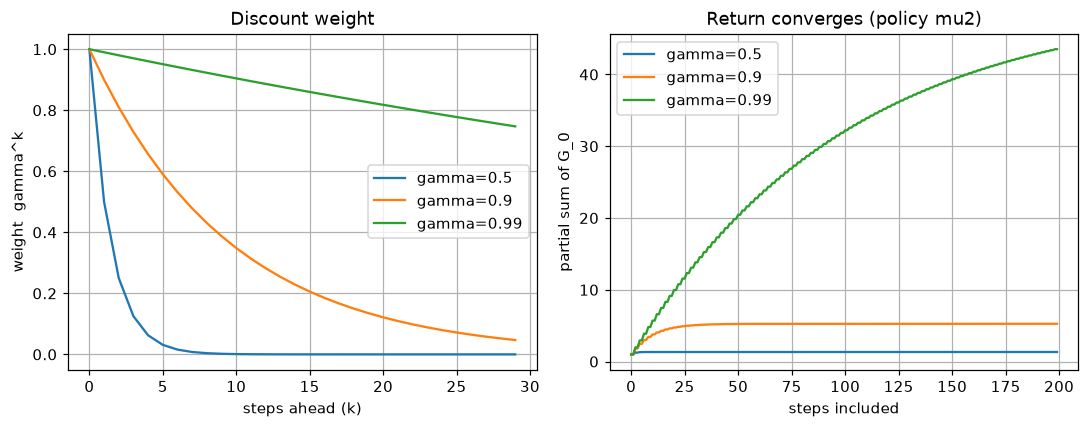
\includegraphics[width=\linewidth]{s02_discount.png}
\caption{할인율의 두 역할. 왼쪽은 가중치 $\gamma^k$ 자체로 유효 지평선에 대응하고, 오른쪽은 수익의
부분합이 수렴하는 모습으로 절단 오차에 대응한다. 왼쪽에서 $\gamma=0.5$는 10걸음이면 사실상 $0$이지만
$\gamma=0.99$는 30걸음까지 $0.74$가 남는다. \texttt{s02\_discount.py}에서 생성.}
\label{fig:discount}
\end{figure}

\subsection{상태 가치 함수}

정책이 확률적이거나 상태 전이가 확률적이면 수익 $G_t$는 매번 다른 값이 나온다. 하나의 숫자로 쓸 수
없으므로 기댓값을 취한다. 이것이 \emph{상태 가치 함수}(state-value function)다.
\begin{equation}
  v_\pi(s) = \E\bigl[G_t \mid S_t=s, \pi\bigr] = \E_\pi\bigl[G_t \mid S_t=s\bigr].
  \label{eq:state-value}
\end{equation}
오른쪽 표기는 조건부의 $\pi$를 기댓값 연산자의 아래첨자로 옮긴 것으로, 뜻은 같다.

식~\eqref{eq:state-value}을 1장의 행동 가치 $q(A)=\E[R\mid A]$와 나란히 놓으면 무엇이 확장되었는지가
분명해진다(표~\ref{tab:q-vs-v}). 밴디트에서는 한 번의 보상을 행동에 대해 평균했지만, MDP에서는 보상의
할인 합을 상태에 대해 평균한다. 그리고 결정적으로, $v_\pi$에는 정책이 붙어 있다. 상태 $s$ 이후의
모든 행동이 $\pi$를 따르므로 정책이 바뀌면 값도 바뀐다. $v_\pi(s)$는 \emph{정책 $\pi$가 상태 $s$에서
받은 성적표}인 셈이다.

\begin{table}[htbp]
\centering
\caption{밴디트의 행동 가치와 MDP의 상태 가치 비교}
\label{tab:q-vs-v}
\small
\begin{tabular}{@{}lll@{}}
\toprule
 & 밴디트(1장) $q(A)$ & MDP(2장) $v_\pi(s)$ \\
\midrule
무엇의 기댓값인가 & 한 번의 보상 $R$      & 수익 $G_t$(보상의 할인 합) \\
무엇의 함수인가   & 행동 $A$              & 상태 $s$ \\
정책의 영향       & 없음(그 행동 한 번뿐) & 있음(이후 모든 행동이 $\pi$를 따름) \\
\bottomrule
\end{tabular}
\end{table}

\subsection{최적 정책과 최적 가치 함수}
\label{sec:optimal-policy}

목표는 가장 좋은 정책을 찾는 것이다. 그런데 상태가 여럿이면 ``가장 좋다''를 정의하는 일부터 간단하지
않다. 그림~\ref{fig:partial-order} 왼쪽처럼 두 정책의 가치 곡선이 여러 번 교차하면, $\texttt{L2}$에서는
$\pi$가 낫고 $\texttt{L5}$에서는 $\pi'$가 나아 우열을 정할 수 없다.

\begin{figure}[htbp]
\centering
\begin{minipage}[t]{0.53\linewidth}\centering
  \includegraphics[width=\linewidth]{{fig 2-10}.png}
\end{minipage}\hfill
\begin{minipage}[t]{0.43\linewidth}\centering
  \includegraphics[width=\linewidth]{{fig 2-11}.png}
\end{minipage}
\caption{두 정책의 비교. 곡선이 교차하면 우열을 정할 수 없고(왼쪽), 모든 상태에서 위에 있을 때만
더 낫다고 정의한다(오른쪽). \bookfig{2-10, 2-11}}
\label{fig:partial-order}
\end{figure}

그래서 정책 사이의 순서를 다음과 같이 \emph{모든 상태에 대한} 조건으로 정의한다.
\begin{equation}
  \pi' \ge \pi
  \quad\stackrel{\text{def}}{\Longleftrightarrow}\quad
  v_{\pi'}(s) \ge v_\pi(s) \quad \text{for all } s \in \Sset.
  \label{eq:policy-order}
\end{equation}
그림~\ref{fig:partial-order} 오른쪽이 이 조건을 만족하는 경우다. 식~\eqref{eq:policy-order}은
\emph{부분 순서}(partial order)이므로, 일반적인 부분 순서 집합이라면 서로 비교 불가능한 원소들만
남아 최댓값이 존재하지 않을 수도 있다.

MDP의 핵심 성질은 그런 일이 일어나지 않는다는 것이다. 즉 어떤 MDP에도 \emph{최적 정책}
$\pi_*$가 적어도 하나 존재하며, 그중에는 결정적 정책이 반드시 있다\cite{sutton}.
그림~\ref{fig:optimal}이 이를 보여준다. 주황색 $\pi_*$는 어떤 상태에서도 다른 정책 아래로 내려가지
않는다.

\begin{figure}[htbp]
\centering
\includegraphics[width=0.52\linewidth]{{fig 2-12}.png}
\caption{최적 정책 $\pi_*$와 그 외 정책들. $\pi_*$는 모든 상태에서 다른 어떤 정책보다 아래에 있지
않다. \bookfig{2-12}}
\label{fig:optimal}
\end{figure}

이때의 가치 함수를 \emph{최적 가치 함수}라 한다.
\begin{equation}
  v_*(s) = \max_{\pi} v_\pi(s), \qquad s\in\Sset.
  \label{eq:optimal-value}
\end{equation}
식~\eqref{eq:optimal-value}에서 $\max$가 각 상태마다 따로 취해졌는데도 그 최댓값들을 \emph{하나의}
정책이 동시에 달성한다는 것이 위 성질의 내용이다. 이 사실은 실용적으로 대단히 중요하다. 덕분에
상태마다 최선의 행동 하나를 적어 둔 표를 찾는 것만으로 문제가 끝나며, 확률적 정책까지 뒤질 필요가
없다.

% =============================================================================
\section{예제: 두 칸짜리 그리드 월드}
% =============================================================================

\subsection{환경}

원서 2.4절이 제시하는 최소 예제를 쓴다. 칸이 둘뿐인 세계다.

\begin{figure}[htbp]
\centering
\includegraphics[width=0.32\linewidth]{{fig 2-13}.png}
\caption{두 칸짜리 그리드 월드. 상태는 $\texttt{L1}, \texttt{L2}$ 둘, 행동은 \texttt{Left},
\texttt{Right} 둘이다. \bookfig{2-13}}
\label{fig:two-square}
\end{figure}

$\texttt{L2}$에는 사과가 놓여 있고, 먹으면 곧바로 다시 생긴다. 종료 상태가 없으므로 이는 지속적
과제다. 양옆은 벽이며, 벽 쪽으로 이동하면 제자리에 머물고 $-1$을 받는다. 표~\ref{tab:two-square-mdp}가
이 MDP의 전부다. 상태 전이 확률이 모두 $1$이므로 환경은 결정적이며, 이하에서는 $\gamma=0.9$를 쓴다.

\begin{table}[htbp]
\centering
\caption{두 칸짜리 그리드 월드의 상태 전이와 보상. \texttt{s01\_mdp.py}의 출력을 옮긴 것이다.}
\label{tab:two-square-mdp}
\small
\begin{tabular}{@{}lllcrl@{}}
\toprule
$s$ & $a$ & $s'$ & $p(s'\mid s,a)$ & $r(s,a,s')$ & 설명 \\
\midrule
\texttt{L1} & \texttt{Left}  & \texttt{L1} & $1.0$ & $-1$ & 벽에 부딪혀 제자리 \\
\texttt{L1} & \texttt{Right} & \texttt{L2} & $1.0$ & $+1$ & 사과를 먹음 \\
\texttt{L2} & \texttt{Left}  & \texttt{L1} & $1.0$ & $0$  & 그냥 이동 \\
\texttt{L2} & \texttt{Right} & \texttt{L2} & $1.0$ & $-1$ & 벽에 부딪혀 제자리 \\
\bottomrule
\end{tabular}
\end{table}

환경은 \texttt{TwoSquareGrid} 클래스가 맡는다. 상태 전이와 보상이 코드~\ref{lst:env}의 두 메서드에
그대로 대응한다.

\begin{lstlisting}[caption={환경 구현 (\texttt{common/two\_square\_grid.py})},label={lst:env}]
def next_state(self, state, action):
    <@\cmt{"""상태 전이 함수 (결정적이므로 다음 상태를 하나만 반환)"""}@>
    if state == 'L1':
        return 'L1' if action == 0 else 'L2'  <@\cmt{\# Left는 벽, Right는 L2로}@>
    else:
        return 'L1' if action == 0 else 'L2'  <@\cmt{\# Left는 L1으로, Right는 벽}@>

def reward(self, state, action, next_state):
    <@\cmt{"""보상 함수 $r(s,a,s')$"""}@>
    if state == next_state:   <@\cmt{\# 벽에 부딪혀 제자리}@>
        return -1.0
    if next_state == 'L2':    <@\cmt{\# 사과가 있는 칸으로 이동}@>
        return 1.0
    return 0.0                <@\cmt{\# L2 -> L1}@>
\end{lstlisting}

\texttt{step()}이 \texttt{done}을 항상 \texttt{False}로 반환한다는 점도 짚어 둘 만하다. 종료 상태가
없는 지속적 과제이므로, 이 환경에서 에피소드의 끝은 존재하지 않고 계산상의 지평선 $N$만이 있다.

\subsection{백업 다이어그램}

상태와 행동의 전이를 나무 모양으로 그린 것을 \emph{백업 다이어그램}(backup diagram)이라 한다.
하얀 원이 상태, 검은 점이 행동, 화살표 옆의 숫자가 보상이다.

\begin{figure}[htbp]
\centering
\begin{minipage}[t]{0.24\linewidth}\centering
  \includegraphics[width=\linewidth]{{fig 2-14}.png}
\end{minipage}\hfill
\begin{minipage}[t]{0.70\linewidth}\centering
  \includegraphics[width=\linewidth]{{fig 2-15}.png}
\end{minipage}
\caption{백업 다이어그램. 결정적 정책은 갈래 없이 한 줄로 내려가지만(왼쪽), 확률적 정책은 한 단계마다
가지가 두 배로 늘어난다(오른쪽). \bookfig{2-14, 2-15}}
\label{fig:backup}
\end{figure}

두 그림의 대비가 상태 가치 함수에 왜 기댓값이 필요한지를 설명한다. 왼쪽처럼 정책과 환경이 모두
결정적이면 궤적이 하나뿐이므로 보상 열을 그대로 더하면 된다. 실제로 그림~\ref{fig:backup} 왼쪽의
수익은 $1+\gamma(-1)+\gamma^2(-1)+\cdots = 1-\gamma/(1-\gamma) = -8$로 계산된다. 그러나 오른쪽처럼
갈래가 생기면 $t$걸음 뒤의 궤적 수가 $2^t$로 늘어나고, 각 궤적에 확률이 붙는다. 이 무수한 궤적을
하나의 숫자로 요약하는 장치가 곧 식~\eqref{eq:state-value}의 기댓값이다.

백업 다이어그램은 다음 장에서 벨만 방정식을 유도할 때 다시 쓰인다. ``한 단계만 내려간 뒤 그 아래는
가치 함수로 대신한다''는 것이 벨만 방정식의 발상이며, 식~\eqref{eq:return-recursive}이 그 재귀 구조를
이미 담고 있다.

\subsection{[보충] 네 정책의 닫힌 형태 해}
\label{sec:closed-form}

이 환경은 상태와 행동이 각각 둘이므로 결정적 정책은 $|\Aset|^{|\Sset|}=2^2=4$가지뿐이다.

\begin{figure}[htbp]
\centering
\includegraphics[width=0.42\linewidth]{{fig 2-16}.png}
\caption{네 가지 결정적 정책. 본고는 이 그림의 번호를 그대로 따른다. \bookfig{2-16}}
\label{fig:four-policies}
\end{figure}

환경과 정책이 모두 결정적이므로 각 정책의 궤적은 하나로 정해지고, 상태 가치를 등비급수로 직접 풀 수
있다. 예컨대 $\mu_2=(\texttt{Right},\texttt{Left})$는 $\texttt{L1}\to\texttt{L2}\to\texttt{L1}\to\cdots$을
반복하며 보상 $1,0,1,0,\dots$를 받으므로
\begin{equation}
  v_{\mu_2}(\texttt{L1}) = 1 + \gamma^2 + \gamma^4 + \cdots = \frac{1}{1-\gamma^2},
  \qquad
  v_{\mu_2}(\texttt{L2}) = \gamma\, v_{\mu_2}(\texttt{L1}) = \frac{\gamma}{1-\gamma^2}
\end{equation}
이다. 나머지도 같은 방식으로 얻어지며, 결과를 표~\ref{tab:closed-form}에 정리하였다.

\begin{table}[htbp]
\centering
\caption{네 정책의 상태 가치. 닫힌 형태에 $\gamma=0.9$를 대입한 값과 $N=500$ 수치
계산(\texttt{s03\_policy\_bruteforce.py})의 결과가 표시된 자릿수에서 완전히 일치한다. 굵게 표시한 것이
최적 정책이다.}
\label{tab:closed-form}
\small
\begin{tabular}{@{}llcccc@{}}
\toprule
\multirow{2}{*}{정책} & \multirow{2}{*}{$(\mu(\texttt{L1}),\mu(\texttt{L2}))$}
& \multicolumn{2}{c}{닫힌 형태} & \multicolumn{2}{c}{$\gamma=0.9$ 수치} \\
\cmidrule(lr){3-4}\cmidrule(l){5-6}
& & $v(\texttt{L1})$ & $v(\texttt{L2})$ & $v(\texttt{L1})$ & $v(\texttt{L2})$ \\
\midrule
$\mu_1$ & (Right, Right) & $1-\dfrac{\gamma}{1-\gamma}$ & $-\dfrac{1}{1-\gamma}$
        & $-8.0000$ & $-10.0000$ \\[2mm]
$\mu_2$ & (Right, Left)  & $\dfrac{1}{1-\gamma^2}$ & $\dfrac{\gamma}{1-\gamma^2}$
        & $\mathbf{5.2632}$ & $\mathbf{4.7368}$ \\[2mm]
$\mu_3$ & (Left, Right)  & $-\dfrac{1}{1-\gamma}$ & $-\dfrac{1}{1-\gamma}$
        & $-10.0000$ & $-10.0000$ \\[2mm]
$\mu_4$ & (Left, Left)   & $-\dfrac{1}{1-\gamma}$ & $-\dfrac{\gamma}{1-\gamma}$
        & $-10.0000$ & $-9.0000$ \\
\bottomrule
\end{tabular}
\end{table}

표~\ref{tab:closed-form}에서 두 가지를 읽을 수 있다.

첫째, 닫힌 형태와 수치 계산이 일치하므로 두 계산 경로가 서로를 검증한다. 이는
식~\eqref{eq:truncation}이 예측한 대로 $N=500$의 절단 오차가 표시 자릿수보다 훨씬 작기 때문이다.

둘째, 최적 정책은 $\gamma$에 의존하지 않는다. $\gamma\in[0,1)$의 모든 값에 대해
\begin{equation}
  v_{\mu_2}(\texttt{L1}) = \frac{1}{1-\gamma^2} \ge 1 \ge 1-\frac{\gamma}{1-\gamma} = v_{\mu_1}(\texttt{L1}),
  \qquad
  v_{\mu_2}(\texttt{L1}) \ge 1 > -\frac{1}{1-\gamma} = v_{\mu_3}(\texttt{L1}) = v_{\mu_4}(\texttt{L1})
\end{equation}
이고, $\texttt{L2}$에서도 $v_{\mu_2}(\texttt{L2})=\gamma/(1-\gamma^2)\ge 0$인 반면 나머지 셋은 모두
$0$ 이하다. 따라서 $\mu_2$는 모든 $\gamma$에서 식~\eqref{eq:policy-order}의 의미로 최적이며, $\gamma>0$
이면 그 우위가 엄격하다. 등호가 성립하는 것은 $\gamma=0$일 때뿐으로, 이때
$\texttt{L1}$에서는 $\mu_1$과 값이 $1$로 같아지고 $\texttt{L2}$에서는 $\mu_4$와 값이 $0$으로 같아진다.

이 등호가 시사하는 바가 작지 않다. $\gamma=0$이면 $G_t=R_t$이므로 두 정책은 첫 보상만 같으면 구별되지
않는다. $\mu_1$이 $\texttt{L2}$에 도착한 뒤 영원히 벽에 부딪힌다는 사실이 $\texttt{L1}$의 점수에 전혀
반영되지 않는 것이다. 표~\ref{tab:gamma-sweep}의 첫 행이 바로 이 현상이다.

\begin{table}[htbp]
\centering
\caption{$\gamma$에 따른 두 정책의 $v(\texttt{L1})$. 수치는 \texttt{s02\_discount.py}의 1,000걸음
계산이다. $\gamma=0.99$에서만 닫힌 형태와 어긋나는데, 이는 1,000걸음이 부족하기 때문이다
(식~\eqref{eq:truncation}의 상한 $0.99^{1000}/0.01\approx4.3\times10^{-3}$).}
\label{tab:gamma-sweep}
\small
\begin{tabular}{@{}lcccc@{}}
\toprule
\multirow{2}{*}{$\gamma$} & \multicolumn{2}{c}{$\mu_2=(\text{Right},\text{Left})$}
& \multicolumn{2}{c}{$\mu_1=(\text{Right},\text{Right})$} \\
\cmidrule(lr){2-3}\cmidrule(l){4-5}
& 닫힌 형태 & 수치(1,000걸음) & 닫힌 형태 & 수치(1,000걸음) \\
\midrule
$0.00$ & $1.0000$  & $1.0000$  & $1.0000$  & $1.0000$  \\
$0.30$ & $1.0989$  & $1.0989$  & $0.5714$  & $0.5714$  \\
$0.50$ & $1.3333$  & $1.3333$  & $0.0000$  & $0.0000$  \\
$0.70$ & $1.9608$  & $1.9608$  & $-1.3333$ & $-1.3333$ \\
$0.90$ & $5.2632$  & $5.2632$  & $-8.0000$ & $-8.0000$ \\
$0.99$ & $50.2513$ & $50.2491$ & $-98.0000$& $-97.9957$\\
\bottomrule
\end{tabular}
\end{table}

표~\ref{tab:gamma-sweep}에서 $\gamma$가 커질수록 두 열의 간격이 벌어진다. $\gamma$는 최적 정책을 바꾸지는
못하지만 \emph{정책 사이의 격차를 드러내는} 역할을 한다. 그리고 격차가 드러나지 않으면 학습 신호도
없다는 점에서, 이는 알고리즘의 관점에서 결코 사소한 차이가 아니다.

\subsection{최적 정책의 전수 탐색}

정책이 네 개뿐이므로 전부 평가해 가장 좋은 것을 고를 수 있다. 아직 벨만 방정식을 도입하지 않았으므로,
가치는 식~\eqref{eq:return}의 정의를 그대로 $N=500$까지 전개해 구한다.

\begin{algorithm}[htbp]
\caption{결정적 정책의 전수 탐색}
\label{alg:bruteforce}
\begin{algorithmic}[1]
\Require MDP $(\Sset,\Aset,p,r)$, 할인율 $\gamma$, 지평선 $N$
\Ensure 최적 정책 $\mu_*$와 최적 가치 $v_*$
\ForAll{$\mu \in \Aset^{\Sset}$} \Comment{결정적 정책 $|\Aset|^{|\Sset|}$가지}
  \ForAll{$s_0 \in \Sset$}
    \State $s \gets s_0$, \; $G \gets 0$
    \For{$k = 0$ \textbf{to} $N-1$}
      \State $s' \gets f(s, \mu(s))$
      \State $G \gets G + \gamma^{k}\, r(s, \mu(s), s')$ \Comment{식~\eqref{eq:return}}
      \State $s \gets s'$
    \EndFor
    \State $v_\mu(s_0) \gets G$
  \EndFor
\EndFor
\State $\mu_* \gets \arg\max_\mu v_\mu(s_0)$ \Comment{임의의 $s_0$ 하나로 충분}
\State \textbf{assert} $v_{\mu_*}(s) \ge v_\mu(s)$ for all $\mu, s$ \Comment{동시 최적성 검증}
\end{algorithmic}
\end{algorithm}

알고리즘~\ref{alg:bruteforce}의 마지막 두 줄이 이 실험의 핵심이다. 최적 정책을 $s_0=\texttt{L1}$ 하나의
기준으로만 뽑아 놓고, 그것이 $\texttt{L2}$에서도 최적인지를 사후에 검증한다. 이는
\S\ref{sec:optimal-policy}에서 서술한
MDP의 성질, 곧 각 상태마다 따로 취한 최댓값을 하나의 정책이 동시에 달성한다는 주장에 대한 직접적인
확인이다. 구현에서는 \texttt{assert} 한 줄이 그 역할을 한다.

\begin{lstlisting}[caption={동시 최적성의 검증 (\texttt{s03\_policy\_bruteforce.py})},label={lst:assert}]
<@\cmt{\# 모든 상태에서 동시에 가장 좋은 정책이 존재한다는 것이 MDP의 중요한 성질이다.}@>
best_policy, best_values = max(results, key=lambda x: x[1]['L1'])
assert all(best_values[s] >= values[s] for _, values in results for s in states), \
    <@\cmt{'모든 상태에서 동시에 최적인 정책이 있어야 한다'}@>
\end{lstlisting}

실행 결과는 표~\ref{tab:closed-form}의 오른쪽 두 열과 같으며, 최적 정책은
$\mu_2=(\texttt{Right},\texttt{Left})$, 최적 가치는 $v_*(\texttt{L1})=5.2632$,
$v_*(\texttt{L2})=4.7368$이다. $\texttt{L1}$에서 오른쪽으로 가 사과를 먹고 $\texttt{L2}$에서 왼쪽으로
돌아와 다시 먹으러 가는 왕복 행동이 최선이라는, 직관과 부합하는 답이다.

\begin{figure}[htbp]
\centering
\includegraphics[width=0.52\linewidth]{{fig 2-17}.png}
\caption{각 정책의 상태 가치 함수. $\mu_2$만이 두 상태 모두에서 나머지보다 위에 있으므로
식~\eqref{eq:policy-order}의 의미로 최적이다. \bookfig{2-17}}
\label{fig:policy-values}
\end{figure}

그림~\ref{fig:policy-values}이 이를 시각화한다. $\mu_2$의 선은 $5.26$에서 $4.74$로 이어지는 반면
나머지 셋은 $-8$과 $-10$ 사이에 모여 있어, 식~\eqref{eq:policy-order}의 조건이 한눈에 확인된다.

\subsection{전수 탐색의 한계}

이 방법은 상태와 행동이 각각 둘이었기 때문에 가능했다. 결정적 정책의 수는
\begin{equation}
  |\Aset|^{|\Sset|}
\end{equation}
로, 상태 수에 대해 지수적으로 늘어난다. 상태가 $100$개, 행동이 $4$개인 평범한 크기의 문제만 해도
$4^{100}\approx1.6\times10^{60}$가지에 이른다. 1초에 $10^{12}$개씩 평가한다 해도 약 $5\times10^{40}$년,
곧 우주 나이의 $10^{30}$배가 걸린다. 전수 탐색은 원리적으로 옳지만 실용적으로 불가능하다.

문제의 구조를 보면 낭비가 어디에 있는지 드러난다. 알고리즘~\ref{alg:bruteforce}은 정책마다 궤적을
처음부터 끝까지 다시 펼치므로, 서로 다른 정책이 공유하는 부분 궤적을 반복해서 계산한다.
식~\eqref{eq:return-recursive}의 재귀 구조를 이용해 이 중복을 제거하는 것이 다음 장의 주제, 곧
벨만 방정식이다.

% =============================================================================
\section{[보충] 할인율이 최적 정책을 바꾸는 경우}
\label{sec:gamma-flip}
% =============================================================================

\S\ref{sec:closed-form}에서 두 칸 세계의 최적 정책이 $\gamma$에 의존하지 않음을 보였다. 이는 편리한
성질이지만 일반적인 사실로 오해해서는 안 된다. 그 세계에서는 두 상태 모두 즉시 보상이 가장 큰 행동이
장기적으로도 최선이어서($\texttt{L1}$에서 \texttt{Right}, $\texttt{L2}$에서 \texttt{Left}), 단기 이득과
장기 이득이 애초에 충돌하지 않았기 때문이다.

충돌이 있는 세계가 이미 이 장의 첫머리에 나와 있다. 그림~\ref{fig:grid-alt}의 배치를 그대로 쓰자.
에이전트는 $\texttt{L3}$에 있고, $\texttt{L1}$에 사과$(+1)$, $\texttt{L4}$에 폭탄$(-2)$,
$\texttt{L5}$에 사과 여섯 개$(+6)$가 있다. 두 걸음 뒤 과제가 끝난다고 보면(일회성 과제) 두 방향의
수익은 다음과 같다.
\begin{align}
  G^{\text{left}}  &= \underbrace{0}_{\texttt{L3}\to\texttt{L2}} + \gamma\underbrace{(+1)}_{\texttt{L2}\to\texttt{L1}} = \gamma, \\
  G^{\text{right}} &= \underbrace{(-2)}_{\texttt{L3}\to\texttt{L4}} + \gamma\underbrace{(+6)}_{\texttt{L4}\to\texttt{L5}} = -2 + 6\gamma.
\end{align}
오른쪽이 유리해지는 조건은 $-2+6\gamma > \gamma$, 즉
\begin{equation}
  \boxed{\;\gamma > \tfrac{2}{5} = 0.4\;}
  \label{eq:gamma-threshold}
\end{equation}
이다. 표~\ref{tab:gamma-flip}이 이를 정리한 것이다.

\begin{table}[htbp]
\centering
\caption{그림~\ref{fig:grid-alt}의 세계에서 $\gamma$에 따른 최적 행동. 임계값
$\gamma=0.4$에서 두 방향의 수익이 $0.4$로 같아지고, 그 위에서 최적 행동이 뒤집힌다.}
\label{tab:gamma-flip}
\small
\begin{tabular}{@{}lccl@{}}
\toprule
$\gamma$ & $G^{\text{left}}=\gamma$ & $G^{\text{right}}=-2+6\gamma$ & 최적 행동 \\
\midrule
$0.0$ & $0.0$ & $-2.0$ & \texttt{Left} \\
$0.2$ & $0.2$ & $-0.8$ & \texttt{Left} \\
$0.4$ & $0.4$ & $\phantom{-}0.4$ & 무차별 \\
$0.6$ & $0.6$ & $\phantom{-}1.6$ & \texttt{Right} \\
$0.9$ & $0.9$ & $\phantom{-}3.4$ & \texttt{Right} \\
\bottomrule
\end{tabular}
\end{table}

식~\eqref{eq:gamma-threshold}의 함의는 두 가지다.

첫째, $\gamma$는 수익을 수렴시키기 위한 기술적 장치가 아니라 \emph{문제의 답을 결정하는 요소}다.
같은 환경, 같은 보상 구조인데도 $\gamma=0.3$인 에이전트와 $\gamma=0.5$인 에이전트는 정반대로 행동한다.
표~\ref{tab:mdp-elements}에서 $\gamma$를 다섯 요소와 따로 적어 둔 것도 이 때문이다. $\gamma$는 환경이
주는 값이 아니라 ``무엇을 목표로 삼을 것인가''를 정하는 설계자의 선택이며, 잘못 고르면 알고리즘이
아무리 정확해도 엉뚱한 정책에 수렴한다.

둘째, 이는 그림~\ref{fig:grid-alt}이 정성적으로 말하던 바에 숫자를 붙인다. ``눈앞의 보상만 보면
틀린다''는 경고에서 ``눈앞''의 범위를 정하는 것이 $\gamma$이고, 그 경계가 이 세계에서는 정확히
$0.4$다. $\gamma=0$인 에이전트는 폭탄만 보고 왼쪽으로 돌아서며, 그 너머의 사과 여섯 개를 영원히
보지 못한다.

% =============================================================================
\section{결론}
% =============================================================================

본고는 마르코프 결정 과정을 통해 상태가 개입하는 강화 학습 문제의 기본 구도를 정리하였다.

MDP는 상태 집합, 행동 집합, 상태 전이 확률, 보상 함수, 정책의 다섯 요소로 정의되며 앞의 넷은 환경,
마지막 하나만이 에이전트의 것이다. 마르코프 성질(식~\eqref{eq:markov})은 다음 상태가 직전의 상태와
행동만으로 정해진다는 요구이며, 세계에 대한 주장이라기보다 상태를 어떻게 설계할 것인가에 대한
지침이다. 목표는 수익(식~\eqref{eq:return})의 기댓값인 상태 가치 함수(식~\eqref{eq:state-value})를
최대화하는 것이고, 정책 사이의 순서는 모든 상태에 대한 조건(식~\eqref{eq:policy-order})으로 정의된다.
부분 순서임에도 최적 정책이 반드시 존재하며 그중에 결정적 정책이 있다는 것이 MDP의 핵심 성질이다.

보충 분석에서 얻은 결론은 다음 세 가지다.

첫째, $\gamma$는 유효 지평선 $1/(1-\gamma)$와 절단 오차 상한 $\gamma^N R_{\max}/(1-\gamma)$라는 두
역할을 동시에 수행하며 둘은 서로 반대 방향으로 작용한다. $\gamma=0.9$, $N=500$인 예제의 절단 오차
상한은 $1.3\times10^{-22}$로 기계 엡실론보다 작아 사실상 무한 걸음과 같다.

둘째, 네 정책의 상태 가치를 닫힌 형태로 유도하여 수치 결과를 독립적으로 검증하였고, 두 칸 세계의
최적 정책 $\mu_2=(\texttt{Right},\texttt{Left})$가 모든 $\gamma\in[0,1)$에 대해 불변임을 보였다.
등호는 $\gamma=0$에서만 성립하는데, 이때 $\mu_1$과 $\mu_2$가 구별되지 않는 것이 근시안적 목표의
전형적인 실패다.

셋째, 그 불변성은 두 칸 세계의 특수성이다. 원서 그림 2-3의 세계에서는 $\gamma=0.4$를 경계로 최적
행동이 뒤집히며, 이는 $\gamma$가 수렴 장치가 아니라 목표 자체를 규정하는 설계 변수임을 보여준다.

한편 본고가 쓴 전수 탐색은 정책 수가 $|\Aset|^{|\Sset|}$로 폭발하므로 이런 최소 예제 밖에서는 쓸 수 없다.
그 낭비의 정체는 정책마다 궤적을 처음부터 다시 펼치면서 공유되는 부분 궤적을 반복 계산한다는 데
있으며, 식~\eqref{eq:return-recursive}의 재귀 구조가 이미 해법을 가리키고 있다. 다음 장에서 이를
\emph{벨만 방정식}으로 정식화하여, 정책을 하나씩 세어 보지 않고 최적 가치를 직접 구하는 방법을
다룬다.

% =============================================================================
\appendix
\section{재현 정보}
% =============================================================================

본고의 모든 수치는 Python 3.12.13, NumPy 2.5.2 환경에서 재현하였다. 예제는 난수를 쓰지 않으므로
시드 고정 없이 항상 같은 값이 나온다.

\begin{table}[htbp]
\centering
\caption{예제 코드 목록. 원서 2장에는 소스 코드가 없으므로 모두 본고의 보충 예제다.}
\label{tab:code}
\small
\begin{tabular}{@{}lll@{}}
\toprule
파일 & 내용 & 대응 절 \\
\midrule
\texttt{common/two\_square\_grid.py}      & \texttt{TwoSquareGrid} 환경                     & \S4.1 \\
\texttt{ch02/s01\_mdp.py}                 & MDP 다섯 요소의 출력, 수익 $G$의 계산과 수렴    & \S2, \S3.2 \\
\texttt{ch02/s02\_discount.py}            & 할인율 $\gamma$의 역할, 가중치와 부분합 그래프  & \S\ref{sec:gamma} \\
\texttt{ch02/s03\_policy\_bruteforce.py}  & 결정적 정책 전수 탐색과 동시 최적성 검증        & \S4.4 \\
\bottomrule
\end{tabular}
\end{table}

표~\ref{tab:horizon}, \ref{tab:truncation}, \ref{tab:closed-form}의 닫힌 형태 열, 그리고
표~\ref{tab:gamma-flip}은 본고를 위해 별도로 계산한 값이다. 나머지 수치는 표~\ref{tab:code}의 예제를
그대로 실행해 얻은 출력이다.

정책의 번호는 본고와 예제 코드 모두 원서 그림 2-16을 따른다. 즉 $\mu_1=(\texttt{Right},\texttt{Right})$,
$\mu_2=(\texttt{Right},\texttt{Left})$이며, \texttt{s02\_discount.py}의 출력에서도 같은 순서로 나열된다.
다만 표~\ref{tab:gamma-sweep}은 최적 정책을 먼저 보이기 위해 $\mu_2$를 왼쪽 열에 두었으므로, 콘솔
출력과 열 순서가 반대라는 점만 유의하면 된다.

\begin{thebibliography}{9}
\bibitem{dlfs4}
사이토 고키, \emph{밑바닥부터 시작하는 딥러닝 4: 파이썬으로 구현하는 강화 학습 알고리즘}, 한빛미디어, 2023.
\bibitem{ch01}
sajacaros, \emph{밴디트 문제와 행동 가치 추정: 탐색과 활용의 절충, 그리고 비정상 환경에서의 갱신 규칙}, 2026.
\bibitem{sutton}
R.~S. Sutton and A.~G. Barto, \emph{Reinforcement Learning: An Introduction}, 2nd ed., MIT Press, 2018.
\end{thebibliography}

\vspace{4mm}
\noindent\rule{\linewidth}{0.4pt}\\
\footnotesize
본 문서에 실린 그림 중 ``원서 그림''으로 표기한 것은 참고문헌~\cite{dlfs4}의 도판이며, 학습 정리 목적으로
인용하였다. 그 밖의 그림과 표는 본고에서 직접 생성한 것이다.

\end{document}
